%% 
%% Copyright 2007-2020 Elsevier Ltd
%% 
%% This file is part of the 'Elsarticle Bundle'.
%% ---------------------------------------------
%% 
%% It may be distributed under the conditions of the LaTeX Project Public
%% License, either version 1.2 of this license or (at your option) any
%% later version.  The latest version of this license is in
%%    http://www.latex-project.org/lppl.txt
%% and version 1.2 or later is part of all distributions of LaTeX
%% version 1999/12/01 or later.
%% 
%% The list of all files belonging to the 'Elsarticle Bundle' is
%% given in the file `manifest.txt'.
%% 

%% Template article for Elsevier's document class `elsarticle'
%% with numbered style bibliographic references
%% SP 2008/03/01
%%
%% 
%%
%% $Id: elsarticle-template-num.tex 190 2020-11-23 11:12:32Z rishi $
%%
%%
\documentclass[preprint,12pt]{elsarticle}

%% Use the option review to obtain double line spacing
%% \documentclass[authoryear,preprint,review,12pt]{elsarticle}

%% Use the options 1p,twocolumn; 3p; 3p,twocolumn; 5p; or 5p,twocolumn
%% for a journal layout:
%% \documentclass[final,1p,times]{elsarticle}
%% \documentclass[final,1p,times,twocolumn]{elsarticle}
%% \documentclass[final,3p,times]{elsarticle}
%% \documentclass[final,3p,times,twocolumn]{elsarticle}
%% \documentclass[final,5p,times]{elsarticle}
%% \documentclass[final,5p,times,twocolumn]{elsarticle}

%% For including figures, graphicx.sty has been loaded in
%% elsarticle.cls. If you prefer to use the old commands
%% please give \usepackage{epsfig}

%% The amssymb package provides various useful mathematical symbols
\usepackage{amssymb}
%% The amsthm package provides extended theorem environments
%% \usepackage{amsthm}

%% The lineno packages adds line numbers. Start line numbering with
%% \begin{linenumbers}, end it with \end{linenumbers}. Or switch it on
%% for the whole article with \linenumbers.
%% \usepackage{lineno}

\usepackage{xcolor}
\usepackage{soul}
\newcommand{\hly}[2][yellow]{{
  \colorlet{foo}{#1}
  \sethlcolor{foo}\hl{#2}}
}
\newcommand{\hlr}[2][red]{{
  \colorlet{foo}{#1}
  \sethlcolor{foo}\hl{#2}}
}
\newcommand{\hlg}[2][green]{{
  \colorlet{foo}{#1}
  \sethlcolor{foo}\hl{#2}}
}
\newcommand{\hlo}[2][orange]{{
  \colorlet{foo}{#1}
  \sethlcolor{foo}\hl{#2}}
}
\newcommand{\hlb}[2][brown]{{
  \colorlet{foo}{#1}
  \sethlcolor{foo}\hl{#2}}
}
\newcommand{\hlgr}[2][lightgray]{{
  \colorlet{foo}{#1}
  \sethlcolor{foo}\hl{#2}}
}

\journal{Lancet Public Health}

\begin{document}

\begin{frontmatter}

%% Title, authors and addresses

%% use the tnoteref command within \title for footnotes;
%% use the tnotetext command for theassociated footnote;
%% use the fnref command within \author or \address for footnotes;
%% use the fntext command for theassociated footnote;
%% use the corref command within \author for corresponding author footnotes;
%% use the cortext command for theassociated footnote;
%% use the ead command for the email address,
%% and the form \ead[url] for the home page:
%% \title{Title\tnoteref{label1}}
%% \tnotetext[label1]{}
%% \author{Name\corref{cor1}\fnref{label2}}
%% \ead{email address}
%% \ead[url]{home page}
%% \fntext[label2]{}
%% \cortext[cor1]{}
%% \affiliation{organization={},
%%             addressline={},
%%             city={},
%%             postcode={},
%%             state={},
%%             country={}}
%% \fntext[label3]{}

\title{Transportation systems and pollution in cities in 2020}

%% use optional labels to link authors explicitly to addresses:
%% \author[label1,label2]{}
%% \affiliation[label1]{organization={},
%%             addressline={},
%%             city={},
%%             postcode={},
%%             state={},
%%             country={}}
%%
%% \affiliation[label2]{organization={},
%%             addressline={},
%%             city={},
%%             postcode={},
%%             state={},
%%             country={}}

\author[melb]{Kerry~A.~Nice\corref{cor1}}
\cortext[cor1]{Principal corresponding author}
\ead{kerry.nice@unimelb.edu.au}
\address[melb]{Transport, Health, and Urban Design Research Lab, Faculty of Architecture, Building, and Planning, University of Melbourne, VIC, Australia.}
%\address[eng]{Melbourne School of Engineering; and Melbourne School of Population and Global Health, University of Melbourne, VIC, Australia.}

%\affiliation{organization={},%Department and Organization
%            addressline={}, 
%            city={},
%            postcode={}, 
%            state={},
%            country={}}

%\begin{abstract}
%% Text of abstract

%\end{abstract}

%%Graphical abstract
%\begin{graphicalabstract}
%\includegraphics{grabs}
%\end{graphicalabstract}

%%Research highlights
%\begin{highlights}
%\item Research highlight 1
%\item Research highlight 2
%\end{highlights}

%\begin{keyword}
%% keywords here, in the form: keyword \sep keyword

%% PACS codes here, in the form: \PACS code \sep code

%% MSC codes here, in the form: \MSC code \sep code
%% or \MSC[2008] code \sep code (2000 is the default)

%\end{keyword}

\end{frontmatter}

%% \linenumbers

%% main text

\section*{Summary}
\textbf{Background} This is the background. It is two sentences.

\textbf{Methods} This is a paragraph of methods.


\textbf{Findings} This is a paragraph of findings.

\textbf{Interpretation} This is the interpretation. It is three sentences.

\textbf{Funding} States the funding sources.

\section*{Research in context}

\textbf{Evidence before this study} 
A paragraph about what existed before.

\textbf{Added value of this study} 
A paragraph about what the study provides.

\textbf{Implications of all the available evidence} 
A paragraph about the implications of the study.

\section*{Introduction}
This has a short introduction, three paragraphs or so.

\section*{Methods}

\subsection*{Data sources}


\begin{figure}
\centering
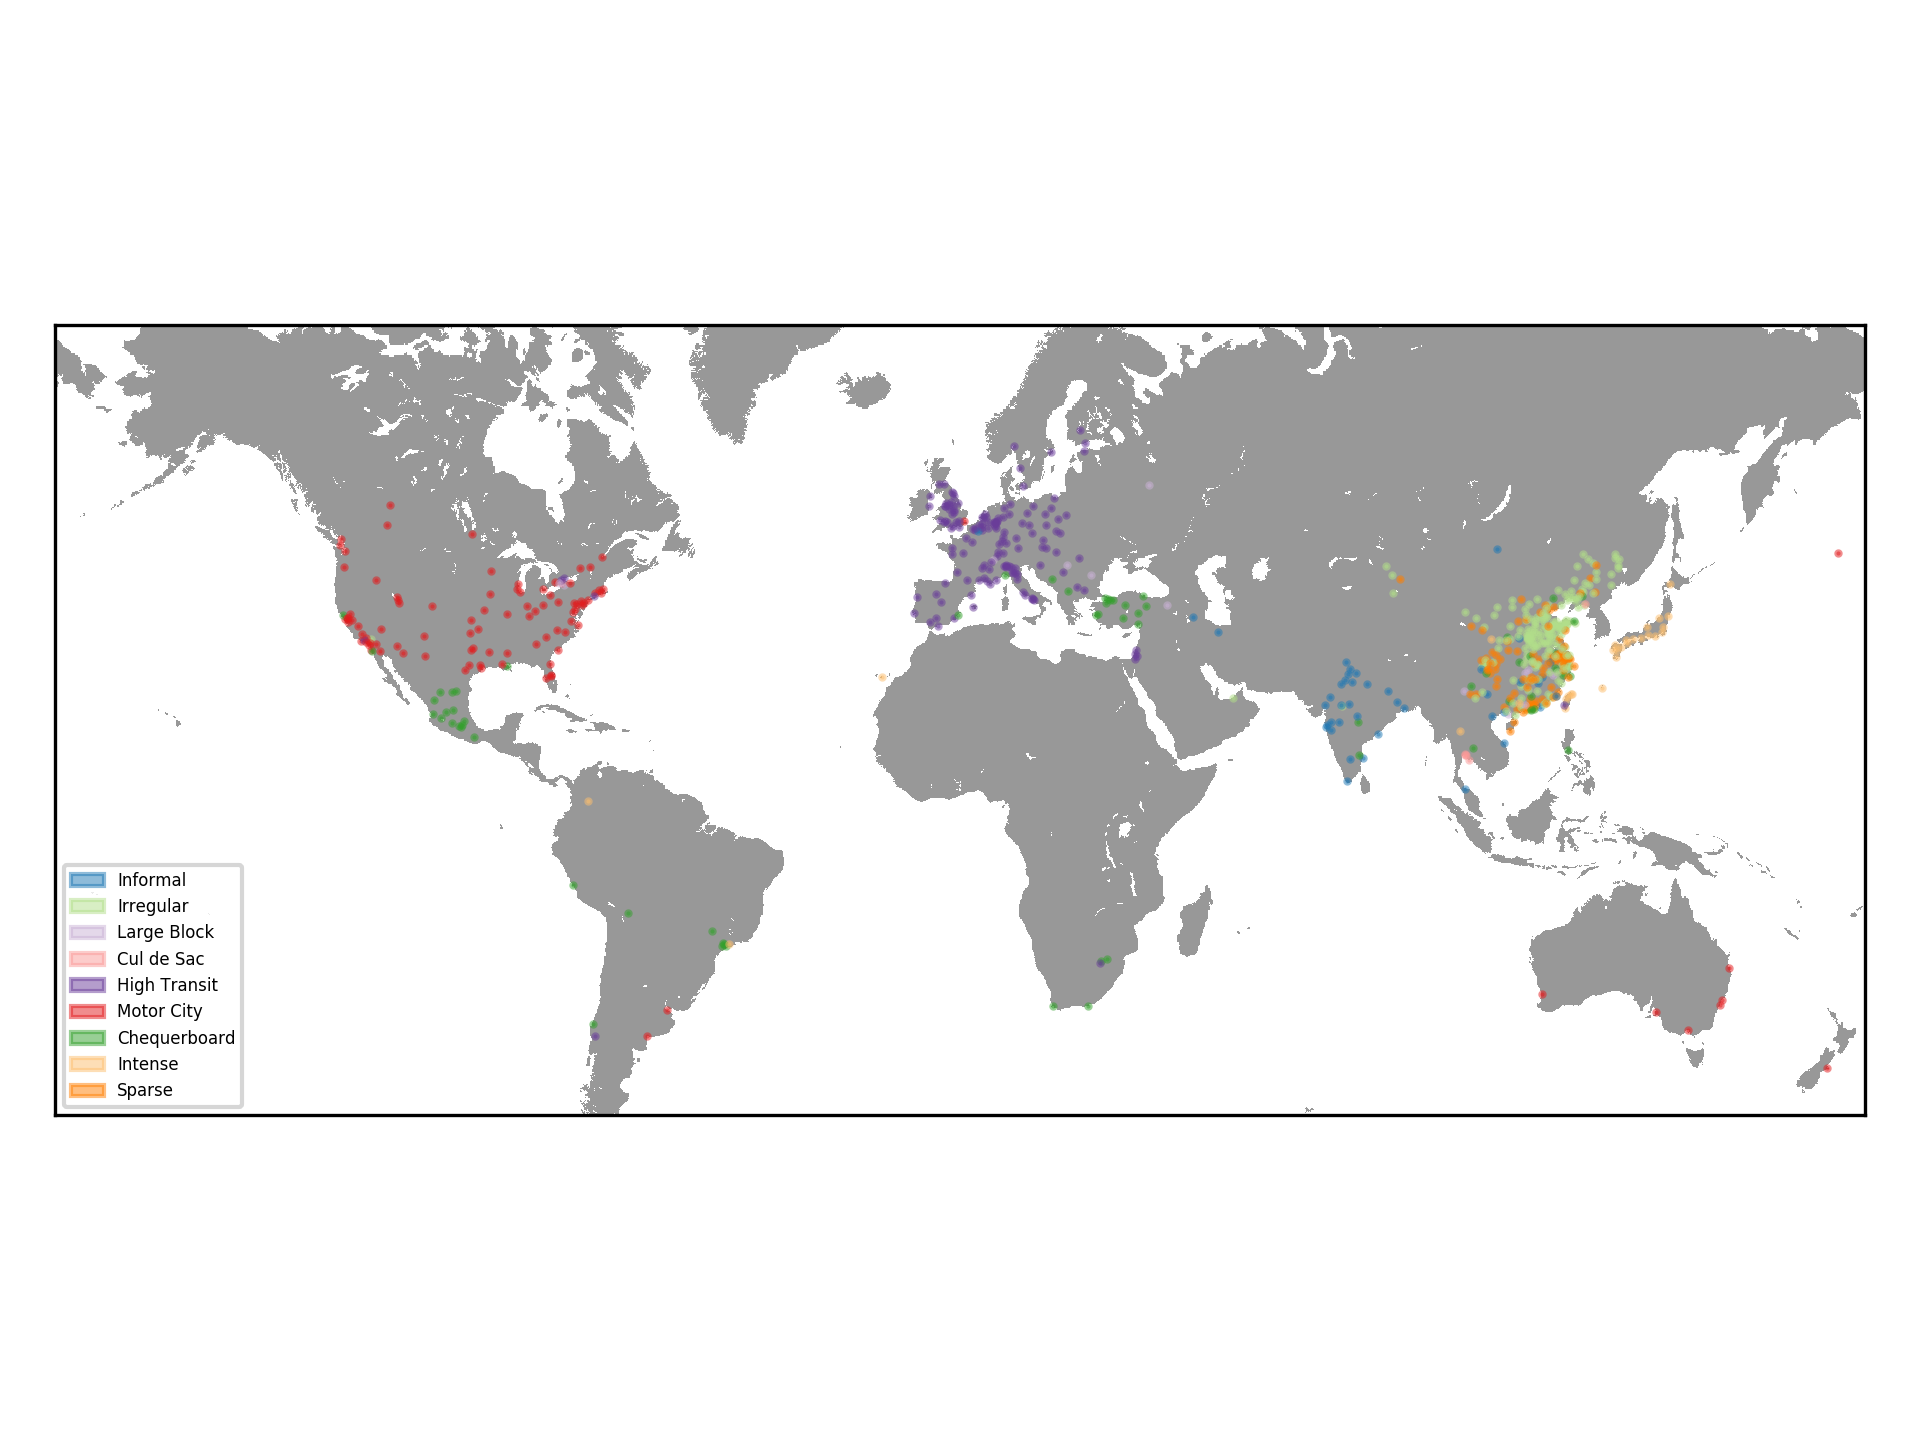
\includegraphics[trim={13 78 13 78},clip,scale=0.9]{Images/WorldPollutionClusters.png}
\caption{\bf Locations and urban typologies of the 679 cities used in this study.}
 \label{fig:clusters}
\end{figure}

Nine global city types were derived in Thompson et al. (2020) \cite{Thompson2020} through visual classification techniques clustering similarities in urban design and transportation networks. These types were defined as high transit (HTR), motor cities (MOT), intense (INT), cul de sac (CUL), Chequerboard (CHQ), informal (INF), irregular (IRR), large block (LBR), sparse (SPR). 

INF cities (n=365) are sparse with low capacity road infrastructure and low amount of formal green space located mostly in Western China and rural India. IRR cities (n=311) have high green space, a mix of formal and high capacity road networks and low mass transit networks and are primary located in Eastern China. LBR cities (n=146) feature medium density formal low and high capacity road networks and medium amount of rail transport and are mostly located in Russia and Eastern Europe. CUL cities (n=26) feature very high density, low capacity mixed formal and informal road networks, with low levels of mass transit and are spread across India, Indonesia, Vietnam, Philippines, and Thailand. HTR cities (n=163) have medium density, high capacity formal road networks with high public transport and are predominately located in Western Europe. MOT cities (n=158) are medium to low density, have high capacity grid based road networks with medium railed transport and are prevalent in North America and Australia. CHQ cities (n=257) are high density, medium capacity mixed formal and informal road networks with medium public transportation and consist of Spanish and Portuguese cities and their colonial cities in Latin America. INT cities (n=22) are very high density, mixed formal high capacity and informal road networks with high public tranport and are mostly Japanese, Columbian, and high density Asian island cities such as Singapore. SPR cities feature low capacity, low density formal and informal road networks with low public transport and are mostly in Western China.



Wijnands et al. (2022) \cite{Wijnands2022} created pollutant and city specific XGBoost models for 679 cities, trained on weather and pollution observations over 2015-2019 and used these models to predict daily pollution levels of NO$_{2}$, PM$_{2.5}$, PM$_{10}$, and O$_{3}$ over 2020. Using 2020 observed values, anomalies were calculated in the absence of a pandemic. The original Thompson et al. (2020) urban typology dataset consisted of the largest 1632 cities in the world. Of these, a subset of 679 cities were used (see Figure \ref{fig:clusters}), those that had pollution data available.

Other datasets:

\textbf{Countermeasures}: A dataset describing coronavirus containment measures taken by governments worldwide on a scale of 0-6. Measures include public gathering cancellations, school closures, non-essential retail closure, curfews, or lockdowns.
https://github.com/OlivierLej/Coronavirus\_CounterMeasures

\textbf{Federal Reserve Bank of Dallas mobility}
https://www.dallasfed.org/research/mei.aspx
The Dallas Fed Mobility and Engagement Index (MEI) summarizes the information in seven different variables based on geolocation data collected from a large sample of mobile devices to gain insight into the economic impact of the pandemic. The MEI measures the deviation from normal mobility behaviors induced by COVID-19. The dataset is based on SafeGraph's Social Distancing Metric database based on mobile phone movements.

\textbf{Descartes mobility:}
[Descartes Labs](https://descarteslabs.com/) is releasing mobility
statistics (representing the distance a typical member of a given
population moves in a day) at the US admin1 (state) and admin2
(county) level.  A technical report describing the motivation behind
this work with methodology and definitions is available at
[arxiv.org/pdf/2003.14228.pdf](https://arxiv.org/pdf/2003.14228.pdf).


\textbf{Baidu mobility: }
Dataset measures number of inner-city journeys in China. This is probably the only mobility dataset for China. It covers January to May 8, 2020 and then Sept 23 through the end of 2020.
https://doi.org/10.7910/DVN/FAEZIO
Hu, T., Guan, W., Zhu, X.,...,  Bao, S. (2020). Building an Open Resources Repository for COVID-19 Research, Data and Information Management (published online ahead of print), 000010247820200012. doi: https://doi.org/10.2478/dim-2020-0012 

\textbf{COVID-19 cases}
This repository attempts to assemble the largest Covid-19 epidemiological database in addition to a powerful set of expansive covariates. It includes open, publicly sourced, licensed data relating to demographics, economy, epidemiology, geography, health, hospitalizations, mobility, government response, weather, and more. Moreover, the data merges daily time-series, +20,000 global sources, at a fine spatial resolution, using a consistent set of region keys.
https://github.com/GoogleCloudPlatform/covid-19-open-data

\textbf{Apple mobility}: Data provided gives the difference in map requests for modes of walking, driving, or public transit over a January 2020 baseline.
https://covid19.apple.com/mobility

\textbf{Google mobility}: Google COVID-19 Community Mobility Reports
Google’s newly released mobility reports, which covers phone-tracking-based changes in mobility across several types of locations, including retail and recreation, grocery stores and pharmacies, parks, transit stations, workplaces, and private residences.
https://www.google.com/covid19/mobility/


\textbf{Stringency: } Oxford COVID-19 Government Response Tracker. The baseline measure of variation in governments' responses is the COVID-19 Government Response Stringency Index. This composite measure is a simple additive score of the seven indicators (S1-S7) measured on an ordinal scale, rescaled to vary from 0 to 100.
https://covidtracker.bsg.ox.ac.uk/


Other possible datasets available to use:

\textbf{International Energy Agency (IEA)}: Global Energy Review 2021. 
Country level energy usage (monthly, 2016-2021) broken down by coal, gas, oil, nuclear, renewable.
Also, Monthly OECD Electricity Statistics. 

\textbf{Ember:} Country level electricity generation (monthly, 2010-2021), broken down by fossil, coal, gas, renewable, etc.
https://ember-climate.org/insights/research/global-electricity-review-2022/
Dataset comprises annual power generation and import data for 209 countries covering the period 2000 to 2020. 

\textbf{Country level CO2 emissions}. (Quarterly, 2001-2021). Australia's is broken down by electricity, stationary, transport, fugitive, industrial, agricultural, waste, land sector.

\textbf{Global Dataset of Human Mobility:} Based on Google Mobility reports.
https://osf.io/rzd8k/




\subsection*{Data analysis}
The methods part 2.



\section*{Results}
Maybe a page of text and some graphs.

Figures \ref{fig:no2} and \ref{fig:pm25} show cumulative anomalies of NO$_{2}$ and PM$_{2.5}$ over 2020. Daily anomalies are a percentage reduction or increase over a January 1-10th, 2020 mean. Cumulative values are calculated as a daily mean across urban typology classes and are a daily summation of previous values across 2020.

Most urban typologies show reductions of NO$_{2}$ at the beginnings of their initial lockdowns. Cities in China in the INF and SPR classes show rapid reductions at the beginning of February, CHQ classes (Turkey, Spain, Latin America) in March and reductions in HTR classes (Western Europe) and MOT (North America and Australia) following in April. Most city classes steadily reduce over 2020 while CHQ show large rapid reductions through the end of the year. INF also shows large reductions over the 2nd half of 2020 but shows some rebounding to normal levels in November and December.

For PM$_{2.5}$, CUL classes show some increases through the first half of 2020 and only begins to reduce in the second half. All other classes show steady reductions through the year, with INT showing the most, followed by LBK, SPR, HTR, INF, IRR and CHQ. MOT reduces the least across the first half of 2020 and shows a large rebound in the 2nd half of the year, quickly exceeding normal levels.

Lots of other metrics are shown in Figure \ref{fig:driving}, presenting mobility and stringency metrics through 2020. (So relate those to how pollution levels evolved over the year.)

Additionally, Tables \ref{tab:no2corr1} through \ref{tab:pm25corr3} show calculated correlations between NO$_{2}$ and PM$_{2.5}$ and mobility metrics for each cluster typology. Three different periods have been calculated: most of 2020, February 15-December 26, 2020, the first half of 2020, February 15-May 1, 2020, and the second half of 2020, July 15-December 26, 2020. (Find which metrics are useful in interpreting the results. And different periods seem to be driven by different factors, so maybe different portions of the year should be looked at differently.)


\begin{figure}
\centering
\includegraphics[trim={0 19 22 43},clip,scale=0.45]{Images/no2CulmReductionClusterMean_2020.png}
\caption{\bf Cumulative daily mean NO$_{2}$ anomalies over 2020 per urban typology type, calculated as a daily percent difference over a January 1-10th, 2020 baseline and summed daily. }
 \label{fig:no2}
\end{figure}

\begin{figure}
\centering
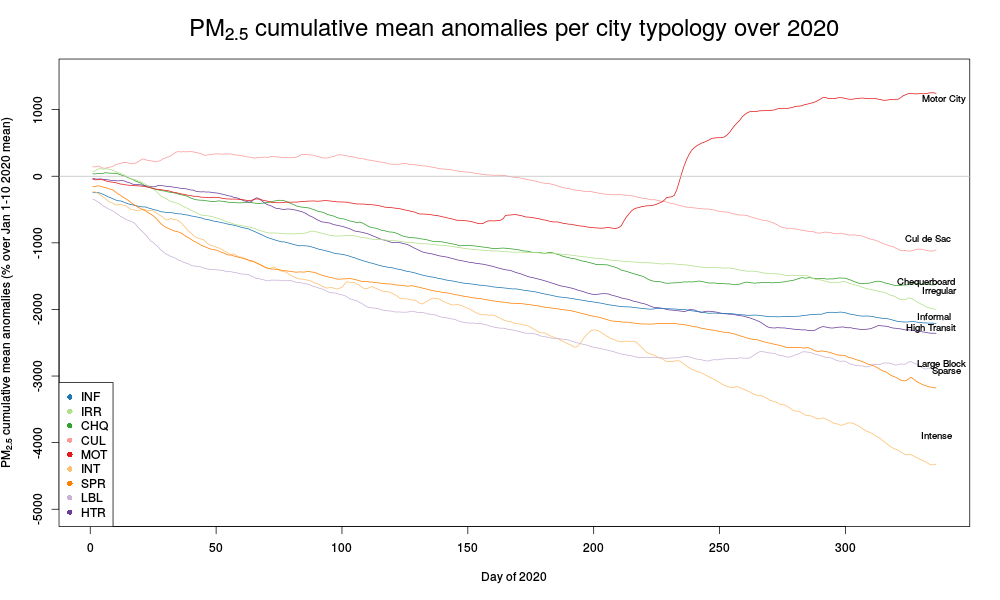
\includegraphics[trim={0 19 22 43},clip,scale=0.45]{Images/pm25CulmReductionClusterMean_2020.png}
\caption{\bf  Cumulative mean PM$_{2.5}$ anomalies over 2020 per urban typology type, calculated as a daily percent difference over a January 1-10th, 2020 baseline and summed daily.}
 \label{fig:pm25}
\end{figure}



%\begin{figure}
%\centering
%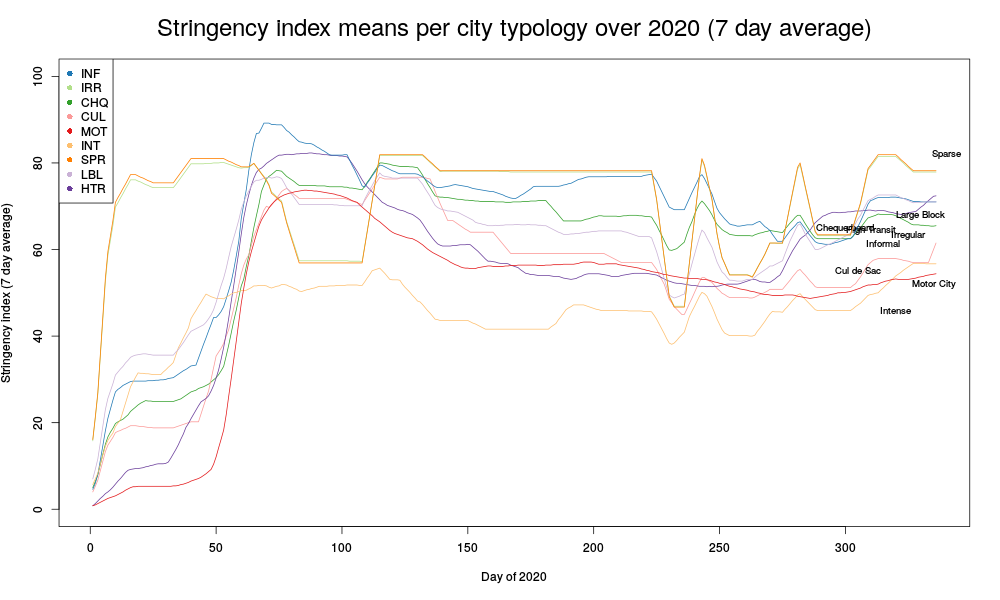
\includegraphics[trim={0 19 22 43},clip,scale=0.25]{Images/LocalStringencyClusterMean7Ave_2020.png}
%\caption{\bf  Stringency index (7 day running average) per urban typology type over 2020.}
% \label{fig:string}
%\end{figure}
%
%\begin{figure}
%\centering
%\includegraphics[trim={0 19 22 43},clip,scale=0.25]{Images/Descarte_mobilityClusterMean7Ave_2020.png}
%\caption{\bf  Descartes mobility index (7 day running average) per urban typology type over 2020.}
% \label{fig:desc}
%\end{figure}
%
%
%
%\begin{figure}
%\centering
%\includegraphics[trim={0 19 22 43},clip,scale=0.25]{Images/CovidCasesClusterMean7Ave_2020.png}
%\caption{\bf  COVID-19 cases per 100,000 (7 day running average) per urban typology type over 2020.}
% \label{fig:covidcases}
%\end{figure}




\begin{figure}
{\tiny a)}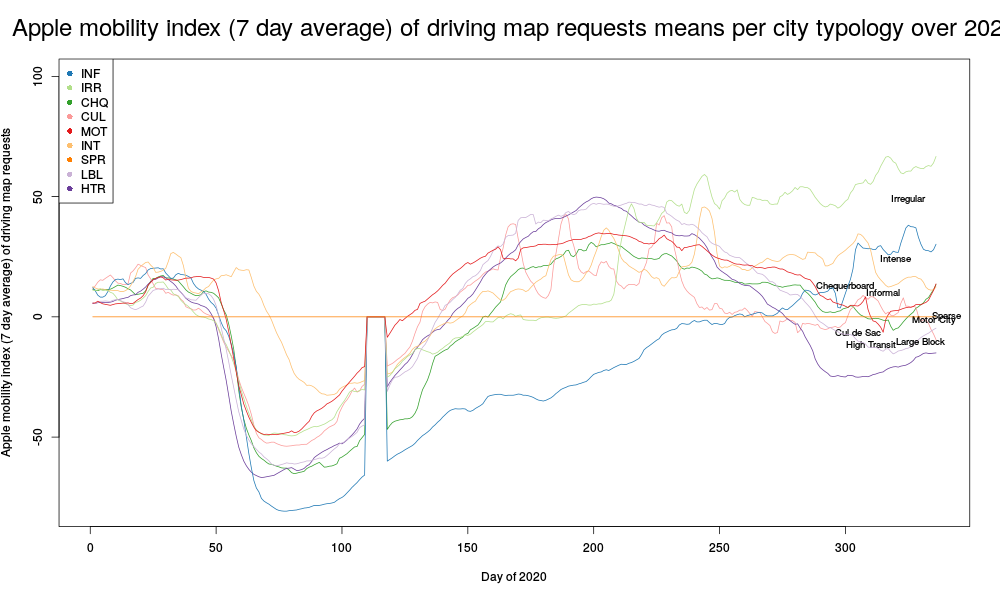
\includegraphics[trim={0 19 22 43},clip,scale=0.23]{Images/AppleDrivingClusterMean7Ave_2020.png}~
{\tiny b)}\includegraphics[trim={0 19 22 43},clip,scale=0.23]{Images/AppleTransitClusterMean_20207Ave.png}
\\
{\tiny c)}\includegraphics[trim={0 19 22 43},clip,scale=0.23]{Images/GoogleTransitClusterMean7Ave_2020.png}~
{\tiny d)}\includegraphics[trim={0 19 22 43},clip,scale=0.23]{Images/GoogleWorkplacesClusterMean7Ave_2020.png}

{\tiny e)}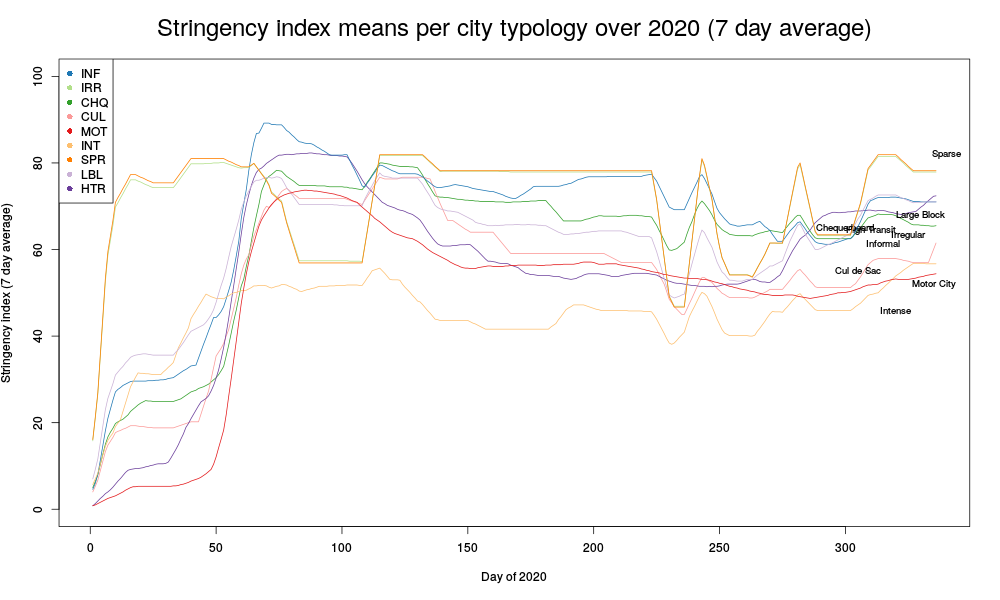
\includegraphics[trim={0 19 22 43},clip,scale=0.23]{Images/LocalStringencyClusterMean7Ave_2020.png}
{\tiny f)}\includegraphics[trim={0 19 22 43},clip,scale=0.23]{Images/Descarte_mobilityClusterMean7Ave_2020.png}
{\tiny g)}\includegraphics[trim={0 19 22 43},clip,scale=0.23]{Images/CovidCasesClusterMean7Ave_2020.png}

\caption{\bf a) Apple mobility index (7 day running average) of map requests for driving directions per urban typology type over 2020. b) Apple mobility index (7 day running average) of map requests for transit directions per urban typology type over 2020. c) Google mobility index (7 day running average) of transit locations per urban typology type over 2020. d) Google mobility index (7 day running average) of workplace locations per urban typology type over 2020. e) Stringency index (7 day running average) per urban typology type over 2020. f) Descartes mobility index (7 day running average) per urban typology type over 2020. g) COVID-19 cases per 100,000 (7 day running average) per urban typology type over 2020.}
 \label{fig:driving}
\end{figure}


\begin{table}[!ht]
\caption{\label{tab:no2corr1} Correlations between NO$_{2}$ anomalies and various mobility indexes over February 15-December 26, 2020.}
    \centering
    \begin{tabular}{|l|p{0.75cm}|p{0.75cm}|p{0.75cm}|p{0.75cm}|p{0.75cm}|p{0.75cm}|p{0.75cm}|p{0.75cm}|p{0.75cm}|}
    \hline
    Typology & CHQ & CUL & HTR & INF & INT & IRR & LBK & MOT & SPR \\ \hline
    Stringency & \hly{.50} & .13 & \hly{.51} & \hlg{.66} & .23 & \hlb{-.40} & .25 & .20 & NaN \\ \hline
    Countermeasures & .26 & .02 & .15 & .14 & .05 & .05 & .30 & .28 & \hlb{-.42} \\ \hline
    Google transit locations & .35 & .12 & .25 & \hly{.53} & .09 & -.30 & .08 & .08 & NaN \\ \hline
    Google workplaces locations & \hlgr{.49} & NaN & \hly{.57} & .00 & -.08 & NaN & .36 & .38 & NaN \\ \hline
    Apple walking requests& \hlgr{.46} & -.01 & \hlgr{.44} & \hlg{.75} & -.17 & .22 & \hlgr{.46} & .17 & NaN \\ \hline
    Apple transit requests& \hlgr{.45} & -.14 & \hly{.50} & \hlg{.71} & -.16 & .22 & \hlgr{.46} & .23 & NaN \\ \hline
    Apple driving requests& -.37 & -.11 & \hlb{-.40} & \hlb{-.44} & -.10 & -.21 & -.05 & -.34 & -.22 \\ \hline
    Covid cases & .18 & .26 & NaN & \hlgr{.47} & -.12 & -.35 & -.21 & NaN & \hlb{-.42} \\ \hline
    Baidu mobility & .02 & NaN & \hlgr{.41} & NaN & NaN & .16 & \hlgr{.44} & .20 & NaN \\ \hline
    Descarte mobility & \hlb{-.41} & -.29 & \hlb{-.45} & \hlr{-.71} & -.03 & \hlo{-.57} & \hlb{-.47} & \hlb{-.49} & \hlo{-.54} \\ \hline
    Dallas Fed mobility & .22 & NaN & .20 & NaN & NaN & -.36 & .09 & .10 & NaN \\ \hline
    \end{tabular}
\end{table}


\begin{table}[!ht]
\caption{\label{tab:no2corr2} Correlations between NO$_{2}$ anomalies and various mobility indexes over February 15-May 1, 2020.}
    \centering
    \begin{tabular}{|l|p{0.75cm}|p{0.75cm}|p{0.75cm}|p{0.75cm}|p{0.75cm}|p{0.75cm}|p{0.75cm}|p{0.75cm}|p{0.75cm}|}
    \hline
    Typology & CHQ & CUL & HTR & INF & INT & IRR & LBK & MOT & SPR \\ \hline
    Stringency & \hlg{.69} & -.03 & \hlg{.65} & \hlg{.73} & \hlgr{.42} & \hlr{-.73} & .21 & \hlg{.62} & .0 \\ \hline
    Countermeasures & \hlo{-.51} & -.03 & -.62 & -.64 & -.1 & -.01 & -.2 & \hlo{-.54} & \hlb{-.45} \\ \hline
    Google transit locations & \hlg{.66} & -.01 & \hly{.58} & \hlg{.71} & .15 & \hlr{-.71} & .2 & \hly{.56} & .0 \\ \hline
    Google workplaces locations & \hlg{.61} & .0 & .64 & \hlg{.61} & .24 & .0 & .28 & \hlg{.65} & .0 \\ \hline
    Apple walking requests & \hlg{.6} & -.04 & \hly{.5} & \hlg{.71} & .24 & \hlr{-.77} & .17 & \hlgr{.44} & .0 \\ \hline
    Apple transit requests & \hlg{.62} & -.04 & \hlr{.61} & \hlg{.71} & .16 & \hlr{-.76} & .19 & \hly{.55} & .0 \\ \hline
    Apple driving requests & \hlr{-.65} & .01 & \hlr{-.62} & \hlr{-.69} & -.17 & \hlo{-.52} & -.15 & \hlr{-.63} & \hlb{-.49} \\ \hline
    Covid cases & \hlb{-.49} & .02 & .0 & \hlgr{.44} & .18 & \hlo{-.59} & .12 & .0 & \hlr{-.75} \\ \hline
    Baidu mobility & .24 & .0 & \hlgr{.49} & .0 & .0 & -.03 & \hlgr{.4} & .29 & .0 \\ \hline
    Descarte mobility & \hlr{-.65} & .01 & \hlr{-.65} & \hlr{-.73} & -.04 & \hlr{-.74} & -.22 & \hlr{-.61} & \hlr{-.78} \\ \hline
    Dallas Fed Mobility & \hly{.52} & .0 & \hly{.57} & .0 & .0 & \hlr{-.74} & .14 & \hly{.55} & .0 \\ \hline
        
    \end{tabular}
\end{table}


\begin{table}[!ht]
\caption{\label{tab:no2corr3} Correlations between NO$_{2}$ anomalies and various mobility indexes over July 15-December 26, 2020.}
    \centering
    \begin{tabular}{|l|p{0.80cm}|p{0.75cm}|p{0.75cm}|p{0.75cm}|p{0.75cm}|p{0.75cm}|p{0.75cm}|p{0.75cm}|p{0.75cm}|}
    \hline
    Typology & CHQ & CUL & HTR & INF & INT & IRR & LBK & MOT & SPR \\ \hline
    Stringency & .10 & .13 & .19 & \hlg{.75} & .04 & .24 & .01 &  -.36 & .0 \\ \hline
    Countermeasures & -.02 & .29 & .0 &  -.3 & .19 &  -.15 & .03 & .21 & .0 \\ \hline        
    Google transit locations & -.1 & .08 &  -.18 & \hlgr{.45} & .01 & .1 &  -.17 &  -.28 & .0 \\ \hline
    Google workplaces locations & .14 & .0 & .33 &  \hlo{-.53} &  -.35 & .0 & .06 &  -.01 & .0 \\ \hline
    Apple walking requests &  -.16 &  -.24 & .15 & \hlg{.8} &  \hlb{-.43} &  -.04 &  -.04 &  \hlb{-.44} & .0 \\ \hline
    Apple transit requests &  -.04 &  -.36 & .2 & \hlg{.76} &  \hlb{-.44} & .03 &  -.05 &  -.36 & .0 \\ \hline
    Apple driving requests &  -.06 & .12 &  -.19 &  -.37 & .01 &  -.25 &  -.09 &  -.21 &  -.21 \\ \hline
    Covid cases &  -.06 & .24 & .0 & \hly{.57} &  -.14 &  -.1 & .0 & .0 &  -.36 \\ \hline
    Baidu mobility &  -.01 & .0 & .07 & .0 & .0 & .26 &  -.05 &  -.04 & .0 \\ \hline
    Descarte mobility & .09 &  \hlb{-.41} & .06 &  \hlr{-.7} & .0 & \hlgr{.43} & .07 &  -.24 & .32 \\ \hline
    Dallas Fed mobility &  -.02 & .0 &  -.34 & .0 & .0 & .04 &  -.18 &  \hlb{-.42} & .0 \\ \hline

    \end{tabular}
\end{table}


\begin{table}[!ht]
\caption{\label{tab:pm25corr1} Correlations between PM$_{2.5}$ anomalies and various mobility indexes over February 15-December 26, 2020.}
    \centering
    \begin{tabular}{|l|p{0.75cm}|p{0.75cm}|p{0.75cm}|p{0.75cm}|p{0.75cm}|p{0.75cm}|p{0.75cm}|p{0.75cm}|p{0.75cm}|}
    \hline
    Typology & CHQ & CUL & HTR & INF & INT & IRR & LBK & MOT & SPR \\ \hline
    Stringency & .16 & -.03 & .13 & \hlgr{.40} & -.16 & \hlb{-.45} & -.09 & -.04 & NaN \\ \hline
    Countermeasures & .26 & .09 & .30 & \hly{.56} & .07 & -.11 & .18 & .01 & -.30 \\ \hline
    Google transit locations & .12 & .05 & .14 & .36 & -.16 & -.37 & -.07 & .04 & NaN \\ \hline
    Google workplaces locations & .10 & NaN & .16 & \hlgr{.42} & -.09 & NaN & .00 & .05 & NaN \\ \hline
    Apple walking requests & .19 & -.16 & .09 & \hly{.50} & -.13 & -.14 & .10 & .26 & NaN \\ \hline
    Apple transit requests & .13 & -.22 & .03 & \hlgr{.49} & -.06 & -.10 & .08 & .23 & NaN \\ \hline
    Apple driving requests & .00 & -.14 & -.12 & -.20 & .01 & -.24 & .14 & .05 & -.19 \\ \hline
    Covid cases & .19 & .09 & NaN & .00 & -.11 & -.37 & .09 & NaN & -.37 \\ \hline
    Baidu mobility & .05 & NaN & .10 & NaN & NaN & .10 & .25 & .12 & NaN \\ \hline
    Descarte mobility & -.22 & .15 & -.25 & -.12 & .02 & -.24 & -.18 & -.05 & -.29 \\ \hline
    Dallas Fed mobility & -.05 & NaN & .13 & NaN & NaN & -.25 & -.07 & .10 & NaN \\ \hline
    \end{tabular}
\end{table}



\begin{table}[!ht]
\caption{\label{tab:pm25corr2} Correlations between PM$_{2.5}$ anomalies and various mobility indexes over February 15-May 1, 2020.}
    \centering
    \begin{tabular}{|l|p{0.75cm}|p{0.75cm}|p{0.75cm}|p{0.75cm}|p{0.75cm}|p{0.75cm}|p{0.75cm}|p{0.75cm}|p{0.75cm}|}
    \hline
      Typology & CHQ & CUL & HTR & INF & INT & IRR & LBK & MOT & SPR \\ \hline
      Stringency & -.02 & .13 & .27 & .31 & -.19 & \hlr{-.69} & \hlb{-.41} & \hlb{-.45} & .0 \\ \hline
      Countermeasures & .13 & -.21 & -.21 & -.28 & .22 & -.03 & .27 & \hlgr{.44} & \hlb{-.41} \\ \hline
      Google transit locations & -.02 & .1 & .25 & .28 & -.25 & \hlr{-.66} & -.37 & \hlb{-.43} & .0 \\ \hline
      Google workplaces locations & -.12 & .0 & .29 & .28 & -.15 & .0 & -.39 & \hlb{-.43} & .0 \\ \hline
      Apple walking requests & -.1 & .15 & .28 & .28 & -.11 & \hlr{-.68} & \hlb{-.45} & -.39 & .0 \\ \hline
      Apple transit requests & -.06 & .11 & .27 & .29 & -.11 & \hlr{-.67} & \hlb{-.44} & -.38 & .0 \\ \hline
      Apple driving requests & .1 & -.18 & -.3 & -.34 & .07 & \hlo{-.54} & \hly{.52} & \hlgr{.47} & \hlo{-.5} \\ \hline
      Covid cases & \hlb{-.46} & .29 & .0 & .23 & .05 & \hlo{-.54} & .08 & .0 & \hlr{-.63} \\ \hline
      Baidu mobility & .04 & .0 & .1 & .0 & .0 & -.09 & .18 & .05 & .0 \\ \hline
      Descarte mobility & .06 & -.09 & -.27 & -.27 & -.01 & \hlo{-.56} & .38 & \hlgr{.46} & \hlo{-.57} \\ \hline
      Dallas Fed Mobility & -.15 & .0 & .23 & .0 & .0 & \hlr{-.64} & -.39 & \hlb{-.46} & .0 \\ \hline
          \end{tabular}
\end{table}



\begin{table}[!ht]
\caption{\label{tab:pm25corr3} Correlations between PM$_{2.5}$ anomalies and various mobility indexes over July 15-December 26, 2020.}
    \centering
    \begin{tabular}{|l|p{0.75cm}|p{0.75cm}|p{0.75cm}|p{0.75cm}|p{0.75cm}|p{0.75cm}|p{0.75cm}|p{0.75cm}|p{0.75cm}|}
        \hline
    Typology & CHQ & CUL & HTR & INF & INT & IRR & LBK & MOT & SPR \\ \hline
    Stringency & .21 & -.03 & -.3 & .35 & -.05 & -.04 & .02 & .17 & .0 \\ \hline
     Countermeasures & .13 & .26 & .3 & .2 & .16 & -.32 & .0 & -.3 & .0 \\ \hline
    Google transit locations & .12 & .11 & -.04 & .24 & -.02 & -.05 & .1 & .12 & .0 \\ \hline
    Google workplaces locations & .19 & .0 & -.24 & -.06 & .04 & .0 & .07 & .26 & .0 \\ \hline
    Apple walking requests & .04 & -.11 & -.27 & .26 & -.02 & -.39 & .0 & .2 & .0 \\ \hline
    Apple transit requests & -.18 & -.14 & -.32 & .22 & .03 & -.23 & -.1 & .17 & .0 \\ \hline
    Apple driving requests & -.14 & .13 & .34 & \hlo{-.51} & -.04 & -.21 & -.19 & -.09 & -.17 \\ \hline
    Covid cases & .34 & -.12 & .0 & .22 & -.15 & -.32 & .28 & .0 & -.24 \\ \hline
    Baidu mobility & .06 & .0 & -.06 & .0 & .0 & .22 & .04 & .04 & .0 \\ \hline
    Descarte mobility & -.18 & .0 & -.09 & .17 & .06 & \hlgr{.49} & -.08 & .15 & .33 \\ \hline
    Dallas Fed Mobility & -.07 & .0 & -.11 & .0 & .0 & .24 & .05 & .14 & .0 \\ \hline      
        \end{tabular}
    \end{table}




\section*{Discussion}
A page or two of discussion (that also includes the conclusion).

\section*{Contributors}\label{sec:credit}
\textbf{KAN}: Conceptualization, Methodology, Software, Formal Analysis, Writing - Original Draft, Writing - Review \& Editing, Visualization.

\section*{Declaration of interests}\label{sec:dec}
We declare no competing interests.

\section*{Acknowledgments}\label{sec:ak}
KAN is supported by NHMRC/UKRI grant (1194959).


%\section{}
%\label{}

%% The Appendices part is started with the command \appendix;
%% appendix sections are then done as normal sections
%% \appendix

%% \section{}
%% \label{}

%% If you have bibdatabase file and want bibtex to generate the
%% bibitems, please use
%%
%%  \bibliographystyle{elsarticle-num} 
%%  \bibliography{<your bibdatabase>}

%% else use the following coding to input the bibitems directly in the
%% TeX file.

\section*{References}\label{sec:ref}
%\begin{thebibliography}{00}

%% \bibitem{label}
%% Text of bibliographic item



\bibliographystyle{elsarticle-num} 
%\bibliography{bib}
\begin{thebibliography}{1}
\expandafter\ifx\csname url\endcsname\relax
  \def\url#1{\texttt{#1}}\fi
\expandafter\ifx\csname urlprefix\endcsname\relax\def\urlprefix{URL }\fi
\expandafter\ifx\csname href\endcsname\relax
  \def\href#1#2{#2} \def\path#1{#1}\fi

\bibitem{Thompson2020}
J.~Thompson, M.~Stevenson, J.~S. Wijnands, K.~A. Nice, G.~D. P.~A. Aschwanden,
  J.~Silver, M.~Nieuwenhuijsen, P.~Rayner, R.~Schofield, R.~Hariharan, C.~N.
  Morrison, {A global analysis of urban design types and road transport injury:
  an image processing study}, Lancet Planetary Health 4 (2020) 32--42.
\newblock \href {https://doi.org/10.1016/S2542-5196(19)30263-3}
  {\path{doi:10.1016/S2542-5196(19)30263-3}}.

\bibitem{Wijnands2022}
J.~S. Wijnands, K.~A. Nice, S.~Seneviratne, J.~Thompson, M.~Stevenson,
  \href{https://doi.org/10.1016/j.apr.2022.101438}{{The impact of the COVID-19
  pandemic on air pollution: A global assessment using machine learning
  techniques}}, Atmospheric Pollution Research 13~(6) (2022) 101438.
\newblock \href {https://doi.org/10.1016/j.apr.2022.101438}
  {\path{doi:10.1016/j.apr.2022.101438}}.


\end{thebibliography}
\end{document}
\endinput
%%
%% End of file `elsarticle-template-num.tex'.
